\documentclass{article}
\usepackage{graphicx}
\usepackage{tikz}
\usepackage{amsmath}
\usepackage{amssymb}
\usetikzlibrary{positioning}

\title{Probability and Machine Learning: \\
       Analyzing the Use of Probability Theory in Naive Bayes Classifiers and Hidden Markov Models}
\author{Badger Code}
\date{\today}

\begin{document}
\maketitle

\section{Introduction}
Probability theory forms the backbone of many machine learning algorithms, providing a powerful framework for modeling uncertainty and making informed decisions. This paper explores the significant role of probability theory in machine learning, with a focus on two popular algorithms: Naive Bayes classifiers and hidden Markov models. We will delve into the principles behind these algorithms, examine their applications, and discuss how probability theory empowers them to handle various real-world problems.

\section{Probability Basics}
Before delving into machine learning algorithms, let's establish the fundamental concepts of probability theory.

\subsection{Probability Distribution}
A probability distribution describes the likelihood of different outcomes in a random experiment. For a discrete random variable $X$, the probability distribution is typically represented as a probability mass function (PMF). For a continuous random variable, it is represented by a probability density function (PDF).

\subsection{Bayes' Theorem}
Bayes' theorem is a fundamental result in probability theory, providing a way to update probabilities based on new evidence. For two events $A$ and $B$, it is expressed as:
\[ P(A|B) = \frac{P(B|A) \cdot P(A)}{P(B)} \]

\subsection{Conditional Probability}
Conditional probability represents the probability of one event occurring given that another event has occurred. For events $A$ and $B$, the conditional probability of $A$ given $B$ is denoted as $P(A|B)$ and is computed as:
\[ P(A|B) = \frac{P(A \cap B)}{P(B)} \]

\section{Naive Bayes Classifiers}
Naive Bayes is a popular machine learning algorithm used for classification tasks. It is based on Bayes' theorem and the assumption of conditional independence among features.

\subsection{Assumptions in Naive Bayes}
The Naive Bayes classifier assumes that the presence of a particular feature in a class is independent of the presence of other features. This conditional independence assumption simplifies the computation of probabilities.

\subsection{Example: Email Spam Classification}
Consider a binary classification task of email spam detection. The Naive Bayes classifier can be trained on a dataset of labeled emails, where features represent the presence or absence of specific words. Given a new email, the classifier calculates the probabilities of it being spam or non-spam (ham) based on the occurrence of these words in spam and ham emails.

\begin{center}
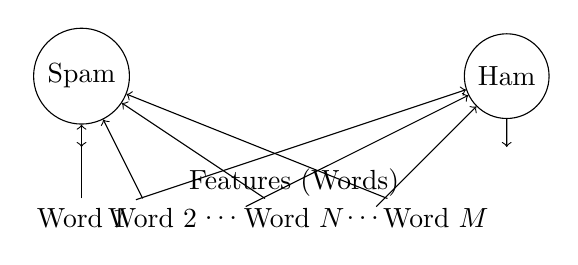
\begin{tikzpicture}[scale=0.9]
    \node[draw, circle] (Spam) at (0,0) {Spam};
    \node[draw, circle] (Ham) at (6,0) {Ham};
    \node[draw=none] (Words) at (3,-1.5) {Features (Words)};

    \draw[->] (Spam) -- (0,-1);
    \draw[->] (Ham) -- (6,-1);

    \node[draw=none] (Word1) at (0,-2) {Word 1};
    \node[draw=none] (Word2) at (1,-2) {Word 2};
    \node[draw=none] (Word3) at (2,-2) {$\dots$};
    \node[draw=none] (Word4) at (3,-2) {Word $N$};
    \node[draw=none] (Word5) at (4,-2) {$\dots$};
    \node[draw=none] (Word6) at (5,-2) {Word $M$};

    \draw[->] (Word1) -- (Spam);
    \draw[->] (Word2) -- (Spam);
    \draw[->] (Word4) -- (Spam);
    \draw[->] (Word6) -- (Spam);

    \draw[->] (Word1) -- (Ham);
    \draw[->] (Word3) -- (Ham);
    \draw[->] (Word5) -- (Ham);
\end{tikzpicture}
\end{center}

In this example, the classifier calculates $P(\text{Spam}|\text{Word 1}, \text{Word 2}, \ldots, \text{Word N})$ and $P(\text{Ham}|\text{Word 1}, \text{Word 2}, \ldots, \text{Word N})$ and assigns the email to the class with higher probability.

\subsection{Advantages and Limitations of Naive Bayes}
Naive Bayes classifiers are computationally efficient, especially for high-dimensional data. However, the conditional independence assumption may not hold in all cases, leading to suboptimal performance.

\section{Hidden Markov Models (HMMs)}
Hidden Markov models are probabilistic models used for sequential data, where the underlying state is not directly observable (hidden).

\subsection{Components of HMM}
An HMM is characterized by three components:
\begin{enumerate}
    \item \textbf{State Space:} A set of hidden states that the model can be in at any given time.
    \item \textbf{Observation Space:} A set of possible observations that can be emitted from each hidden state.
    \item \textbf{Transition and Emission Probabilities:} Probabilities that govern the transitions between hidden states and the emission of observations from states, respectively.
\end{enumerate}

\subsection{Example: Part-of-Speech Tagging}
In natural language processing, HMMs are used for part-of-speech (POS) tagging. Given a sequence of words in a sentence, the HMM predicts the sequence of POS tags for each word.

\subsection{Advantages and Limitations of HMMs}
HMMs are effective for modeling sequential data and are widely used in speech recognition, bioinformatics, and natural language processing. However, they assume that the system satisfies the Markov property, which may not always be accurate.

\section{Conclusion}
Probability theory plays a central role in machine learning algorithms like Naive Bayes classifiers and hidden Markov models. These algorithms leverage probability theory to make informed decisions under uncertainty and handle real-world problems effectively. The principles behind probability theory enable the development of powerful and versatile machine learning models that find applications in diverse fields, making them invaluable tools in the ever-expanding realm of artificial intelligence.

\end{document}